\chapter{Problemanalyse und Stand der Technik}
\label{cha:problemanalyse-stand-der-technik}

Dieses Kapitel beleuchtet die Problemstellung detailliert. Es analysiert sowohl die aktuell eingesetzte Lösung als auch gängige Methoden in Forschung und kommerziellen Anwendungen.

\section{Analyse des aktuell eingesetzten Systems}
\label{sec:analyse-des-akutell-eingesetzten-systems}

\subsection{Architektur und Funktionsweise}
\label{subsec:architektur-und-funktionsweise}

Das bestehende System nutzt Zonal-\gls{OCR} zur Dokumentenverarbeitung \parencite{multidata_help}. 
Vorlagen mit Bounding Boxes definieren die zu erfassenden Zonen. 
Nutzer*innen erstellen für jedes Dokumentenlayout eine Vorlage mit vier Hauptkomponenten:

\begin{itemize}
	\item Suchfelder: Diese legen Position, Bezeichnung und Typ der zu extrahierenden Daten fest.
	\item Identifikationsmerkmale: Sie bestimmen die Position und den spezifischen Text zur Dokumentenerkennung.
	\item Dokumententyp: Er ordnet das Dokument einer bestimmten Kategorie zu (z.B. Rechnung oder Bestellung).
	\item Zusatzinformationen: Diese enthalten relevante Daten für die Weiterverarbeitung.
\end{itemize}

\begin{figure}
	\centering
	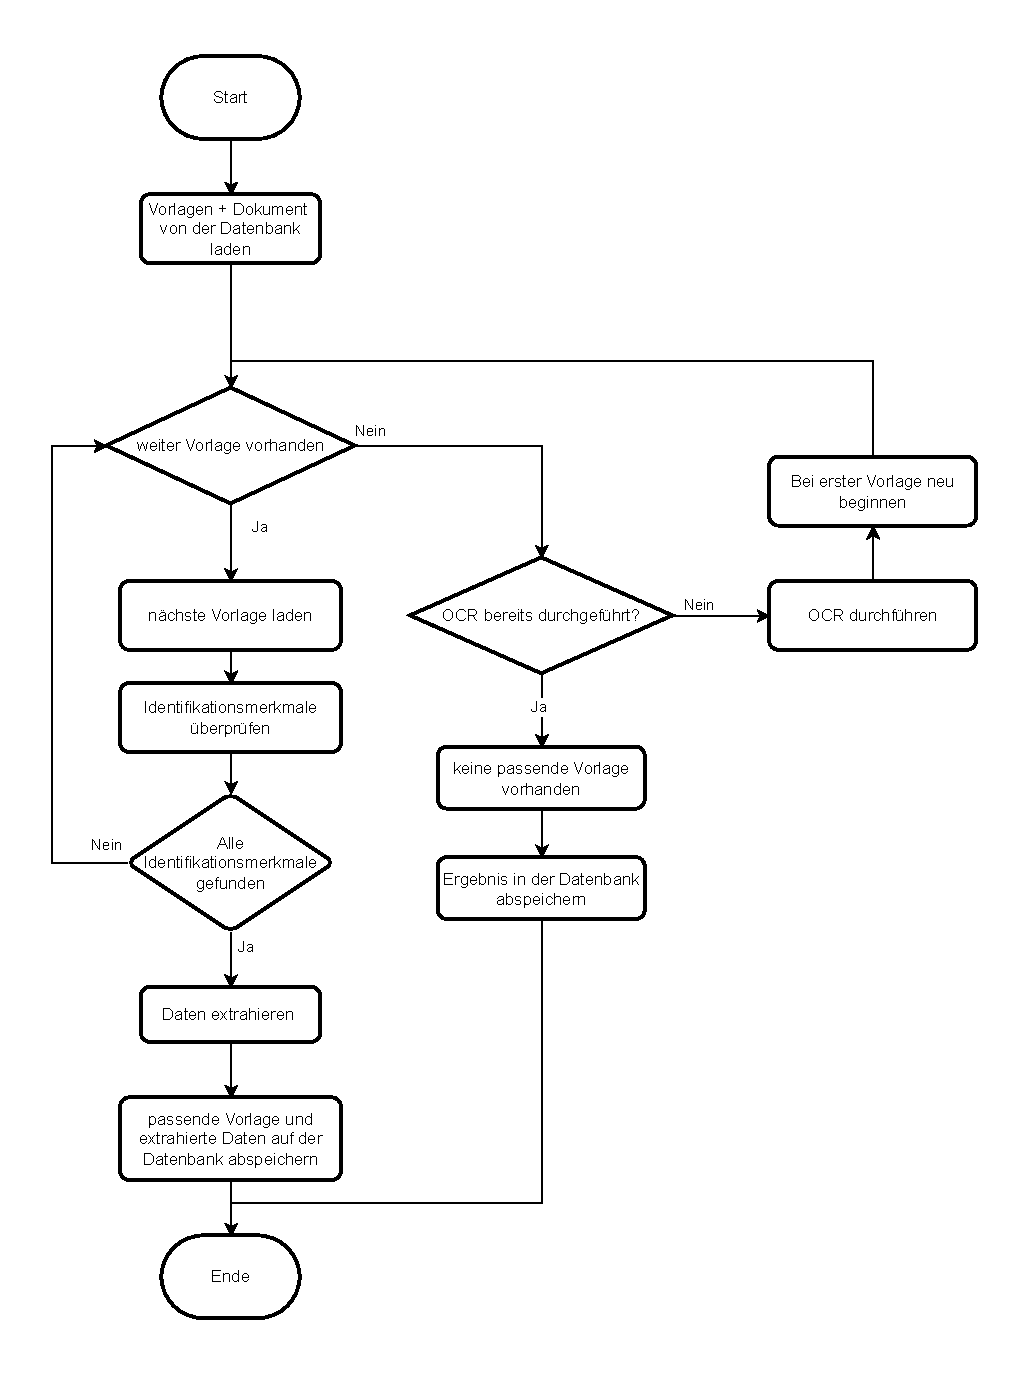
\includegraphics[width=\textwidth]{images/AuswertungBestehendesSystem.drawio.pdf}
	\caption{Ablaufdiagramm des bestehenden Systems}
	\label{fig:auswertung-bestehendes-system}
\end{figure}

Bei der Analyse neuer Dokumente vergleicht das System alle Vorlagen mit den Identifikationsmerkmalen. Bei einer Übereinstimmung extrahiert es die Daten aus den Suchfeldern und identifiziert den Dokumententyp sowie die Zusatzinformationen. Diese Typbestimmung steuert die nachfolgende Datenverarbeitung. Um Ressourcen zu schonen, versucht das System zunächst, eine Vorlage ohne \gls{OCR} zu finden. Scheitert dies, wendet es Tesseract-\gls{OCR} an, um den Text in Bildern zu erfassen, und wiederholt die Suche. Abbildung~\ref{fig:auswertung-bestehendes-system} visualisiert diesen Prozess. Kapitel \ref{subsec:tesseract-ocr} beschreibt das verwendete Tesseract \gls{OCR}-System detaillierter.

\subsection{Stärken und Schwächen}
\label{subsec:stärken-und-schwächen}

Das System überzeugt durch seinen einfachen Aufbau und arbeitet bei wenigen Vorlagen sehr effizient. Ein wesentlicher Vorteil liegt in der Fähigkeit, PDF-Dokumente mit bereits maschinenlesbarem Text ohne \gls{OCR} auszuwerten, was die Verarbeitungszeit erheblich reduziert. Erfahrungen zeigen, dass ein Großteil der zu verarbeitenden Dokumente im PDF-Format vorliegt. Allerdings enthalten viele dieser Dokumente trotz digitaler Erstellung Bilder mit relevantem Text, wodurch \gls{OCR} häufig notwendig bleibt.

Die sequenzielle Suche nach passenden Vorlagen führt zu einer linearen Skalierung der Laufzeit mit der Anzahl der definierten Vorlagen. Der wirtschaftlich bedeutendste Nachteil besteht im hohen manuellen Aufwand für die Definition einer Vorlage für jedes zu verarbeitende Dokumentenlayout. Dieser Aufwand steigt bei Dokumenten mit variabler Form, wie beispielsweise Rechnungen mit unterschiedlichen Positionsauflistungen, da das koordinatenbasierte System hier an seine Grenzen stößt.

Zudem eignet sich das System nicht für die zuverlässige Verarbeitung von Bildern mit schlechter Qualität, Verzerrungen oder Rotationen. Diese Einschränkungen in der Verarbeitbarkeit und mangelnde Flexibilität bei der Bildaufnahme erhöhen den manuellen Korrekturaufwand und erfordern erhöhte Sorgfalt bei der Dokumentenerfassung.

\section{Stand der Technik in der automatisierten Dokumentenverarbeitung}
\label{sec:stand-der-technik-in-der-automatisierten-dokumentenverarbeitung}

\subsection{Traditionelle Methoden der Dokumentenextraktion}
\label{subsec:traditionelle-Methoden-der-Dokumentenverarbeitung}

Historisch entwickelten Forscher*innen Ansätze zur Dokumentenextraktion hauptsächlich auf Basis von Vorlagen oder Regeln, die Kapitel \ref{subsubsec:regelbasierte-ansätze} detailliert erläutert \parencite{YeYibin2018Auso, ChowdhuryGobindaG.1999Tmfi}. Grundlegend für viele dieser Ansätze ist der Fortschritt der \gls{OCR}-Technik, die Kapitel \ref{sec:optical-character-recognition-ocr} beschreibt.

Alternativ kommen auch NLP-basierte Ansätze zum Einsatz \parencite{ChowdhuryGobindaG.1999Tmfi, MarinaiS.2005Annf}. Diese nutzen linguistische Analyse zur Informationsextraktion aus Texten, wobei Techniken wie Named Entity Recognition oder Part-of-Speech Tagging Anwendung finden. Herausforderungen bei der Implementierung NLP-basierter Dokumentenextraktionssysteme liegen vor allem in der Verarbeitung domänenspezifischer Sprache und der Kontextabhängigkeit von Textteilen.

Der Einsatz dieser Techniken kann Schwierigkeiten bezüglich der Skalierbarkeit auf große und diverse Dokumentmengen mit sich bringen \parencite{ChowdhuryGobindaG.1999Tmfi, YeYibin2018Auso}. Die Vorteile dieser Methoden liegen hauptsächlich in der guten Leistung bei bekannten, konsistenten Dokumentenlayouts sowie der Interpretierbarkeit und relativ einfachen Nachvollziehbarkeit der Extraktionslogik. Zudem benötigen sie im Vergleich zu Machine-Learning-Ansätzen weniger Trainingsdaten \parencite{ChowdhuryGobindaG.1999Tmfi, MarinaiS.2005Annf}.

\subsection{Deep-Learning-Ansätze}
\label{subsec:deep-learning-ansätze}

Deep Learning Ansätze revolutionierten in den letzten Jahren die Dokumentenverarbeitung. Im Gegensatz zu traditionellen regelbasierten Techniken lernen Deep-Learning-Modelle komplexe Muster direkt aus den Daten \parencite{YangXiao2017LtES, XuYiheng2020LPoT}.

Entscheidend für diese Entwicklung war die Erforschung von Fully Convolutional Neural Networks (FCN) für die pixelweise Segmentierung von Dokumenten \parencite{YangXiao2017LtES}. FCNs ermöglichen eine Ende-zu-Ende-Verarbeitung vom Eingabebild zur semantischen Segmentierung.

Innovative multimodale Ansätze wie MFCN \parencite{YangXiao2017LtES} und LayoutLM \parencite{XuYiheng2020LPoT} integrieren visuelle und textuelle Informationen in einem gemeinsamen Modell. Durch die Kombination von Bild- und Textmerkmalen erfassen diese Architekturen sowohl das Layout als auch den Inhalt von Dokumenten.

Die Vorteile von Deep-Learning-Ansätzen liegen vor allem in der automatischen Merkmalsextraktion, der verbesserten Verarbeitung komplexer Layouts und der gleichzeitigen Erkennung visueller und semantischer Klassen. Dies ermöglicht Spitzenleistungen bei verschiedenen Dokumentenverständnisaufgaben \parencite{YangXiao2017LtES, XuYiheng2020LPoT}. Die Nachteile dieser Technik bestehen hauptsächlich im hohen Bedarf an annotierten Trainingsdaten sowie der Komplexität der Modelle und dem damit verbundenen Rechenaufwand beim Training \parencite{YangXiao2017LtES, XuYiheng2020LPoT}.

\subsection{OCR-freie Document-Transformer}
\label{subsec:ocr-freie-document-transformer}

Die meisten aktuellen Methoden zur Umsetzung von Informationsextraktionsaufgaben nutzen \gls{OCR}-Methoden, um visuelle Dokumente in Text und teilweise auch in Layoutinformationen vorzuverarbeiten \parencite{KimGeewook2022ODUT}. Dieser Vorverarbeitungsschritt bringt in der Regel einen hohen Rechenaufwand sowie eingeschränkte Flexibilität bei verschiedenen Sprachen mit sich. Zudem setzen sich Fehler, die beim \gls{OCR}-Prozess auftreten, im nachfolgenden Datenextraktionsschritt fort.

Um diese Probleme zu minimieren, entwickelten Forscher*innen mit \gls{DONUT} ein End-to-End-Modell, das das Eingangsbild direkt in strukturierte Daten verarbeitet \parencite{KimGeewook2022ODUT}. Wie Abbildung \ref{fig:donut-comparison} zeigt, bringt dies sowohl Verbesserungen bezüglich des Ressourcenbedarfs als auch bei der Genauigkeit. Zusätzlich kann dieses Modell auch die Klassifizierung der Dokumente vornehmen, wodurch keine zusätzliche Komponente zur Klassifizierung notwendig wird.

\begin{figure}[htb]
	\centering
	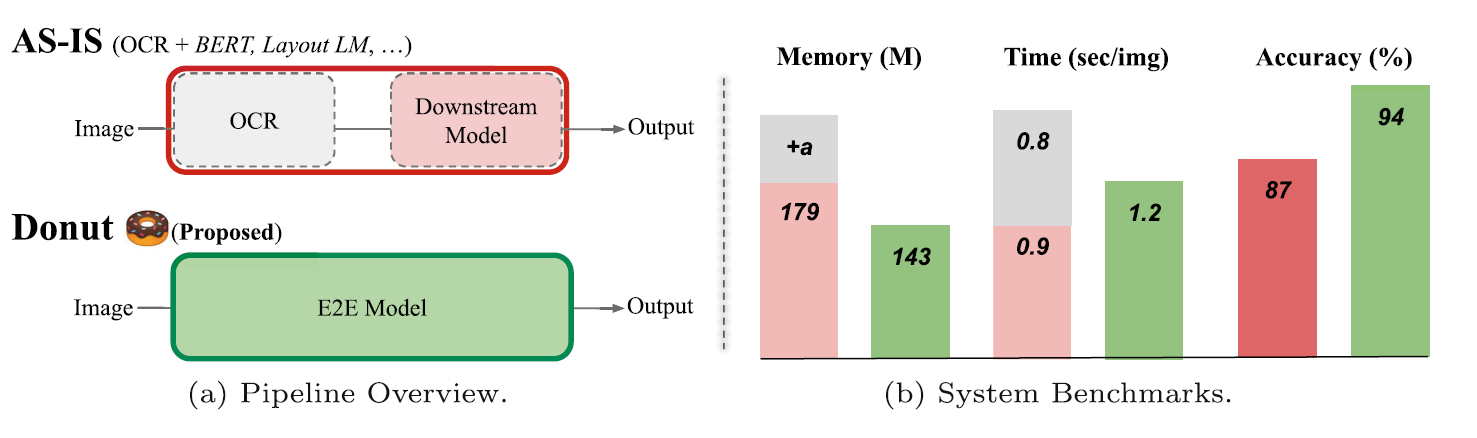
\includegraphics[width=\textwidth]{images/Donut_comparison.png}
	\caption{Vergleich des Ressourcenverbrauchs, der Performanz und Genauigkeit zwischen \gls{DONUT} und \gls{OCR}-basierten Ansätzen \parencite{KimGeewook2022ODUT}}
	\label{fig:donut-comparison}
\end{figure}

\subsection{Language-Model-Prompting-basierte Document Information Extraction}
\label{subsec:language-model-basierte-document-information-extraction}

Ein weiterer vielversprechender Ansatz der Dokumentenextraktion nutzt die großen Fortschritte bei der Entwicklung von \glspl{LLM}. Forscher*innen bezeichnen die Methode als \gls{LMDX} und verwenden Prompting, um die Extraktion von Informationen aus visuell anspruchsvollen Dokumenten mithilfe von \glspl{LLM} zu ermöglichen \parencite{PerotVincent2024LLMD}.

Der \gls{LMDX}-Ansatz, wie von \textcite{PerotVincent2024LLMD} beschrieben, besteht aus vier Hauptschritten:

\begin{enumerate}
	\item Chunking: Ein Algorithmus zerlegen das Dokument in kleinere Teile, die das \gls{LLM} verarbeiten kann.
	\item Prompt-Generierung: Für jeden Chunk wird ein Prompt erstellt, der den Dokumenteninhalt, eine Aufgabebeschreibung und das Zielschema enthält.
	\item \gls{LLM}-Inferenz: Das \gls{LLM} generiert Vervollständigungen basierend auf den Prompts.
	\item Dekodierung: Die \gls{LLM}-Ausgaben werden in strukturierte Entitäten und deren Positionen im Dokument umgewandelt.
\end{enumerate}

Ein wichtiges Element von \gls{LMDX} sind Koordinaten-Token, die das System verwendet, um Layoutinformationen auf textbasierte Weise an das \gls{LLM} zu übermitteln. Dadurch kann das \gls{LLM} auch das Layout des Dokuments berücksichtigen \parencite{PerotVincent2024LLMD}. LLM-Prompting-basierte Parser eignen sich sowohl für die Datenextraktion als auch die Kategorisierung von Dokumenten. Die genaue Implementierung eines \gls{LMDX}-basierten Dokumentenverarbeitungssystems beschreibt Kapitel ... .

Die Vorteile von \gls{LMDX} liegen vor allem in seiner Flexibilität und der Unterstützung für die Extraktion von einzelnen, wiederholten und hierarchischen Entitäten. Außerdem ermöglicht es die Lokalisierung der extrahierten Entitäten im Dokument. Auch die Möglichkeit zur Zero-Shot-Extraktion ohne Trainingsprozess und die hohe Dateneffizienz bei der Anpassung an neue Dokumententypen sind besonders vorteilhaft für die Problemstellung. Die Nachteile bei der Verwendung hingegen liegen vor allem im relativ großen Rechenaufwand, den viele \glspl{LLM} verursachen. Zudem neigen \glspl{LLM} dazu, Informationen zu ``halluzinieren'', was die Zuverlässigkeit der Extraktion beeinträchtigen kann.

Tests und Benchmarks wie VRDU \parencite{WangZilong2023VABf} und CORD \parencite{park2019cord} zeigen, dass \gls{LMDX} den aktuellen Stand der Technik in verschiedenen Disziplinen der Dokumentenverarbeitung übertrifft oder zumindest eine robuste Lösung darstellt \parencite{PerotVincent2024LLMD}. Die konkreten Werte im Vergleich mit anderen Modellen sind in der Tabelle \ref{tab:lmdx_cord_zero_shot_results} ersichtlich.

\begin{table}
	\centering
	\begin{tabular}{lcc}
		\hline
		Modell & Modalität & Micro-F1 \\
		\hline
		LLaVA-v1.5-13B & I & 5.97 \\
		GPT-4V$_\text{+Image}$ & I & 64.05 \\
		Gemini Pro$_\text{+Image}$ & I & 47.12 \\
		Gemini Pro$_\text{+OCR}$ & T & 59.57 \\
		PaLM 2-S$_\text{+OCR}$ & T & 55.85 \\
		GPT-3.5$_\text{+OCR}$ & T & 48.92 \\
		LMDX$_\text{PaLM 2-S}$ & T+L & \textbf{66.95} \\
		LMDX$_\text{Gemini Pro}$ & T+L & \underline{66.03} \\
		\hline
	\end{tabular}
	\caption{Micro-F1-Wert verschiedener Sprachmodell-basierten Dokumentenverarbeitungstechniken von Zero-Shot-Tests anhand des CORD \parencite{park2019cord} Datensatzes, durchgeführt durch \textcite{PerotVincent2024LLMD} (T → Text, L → Layout, I → Image)}
	\label{tab:lmdx_cord_zero_shot_results}
\end{table}

\subsubsection{Verwendung multimodaler \glspl{LLM}}
\label{subsec:verwendung-multimodaler-llms}

Bei der Verarbeitung visueller Dokumente eignen sich besonders multimodale \glspl{LLM}, da diese die Bilder direkt verarbeiten können, ohne einen \gls{OCR}-Schritt und die damit verbundene Darstellung des Layouts in Textform zu benötigen.

Einige Beispiele für multimodale \glspl{LLM}, die für Dokumentenverständnis geeignet sind:

\begin{enumerate}
	\item DocLLM \parencite{WangDongsheng2023DAlg}: Ein dokumentenzentriertes \gls{LLM}, das Informationsextraktion als Frage-Antwort-Aufgabe formuliert. Es ermöglicht Zero-Shot-Extraktion, hat jedoch Einschränkungen bei der Lokalisierung und der Extraktion hierarchischer Entitäten.
	\item LLaVA \parencite{CaffagniDavide2024WHRG}: Ein multimodales Modell, das Bild- und Texteingaben verarbeiten kann. Obwohl es nicht speziell für Dokumentenverarbeitung entwickelt wurde, zeigt es Potenzial für dokumentenbezogene Aufgaben.
	\item GPT-4V \parencite{openai_chatgpt} oder Claude \parencite{anthropic_claude}: Diese fortgeschrittenen multimodalen Modelle von OpenAI bzw. Anthropic können Bild- und Texteingaben verarbeiten und zeigen vielversprechende Ergebnisse bei verschiedenen dokumentenbezogenen Aufgaben.
\end{enumerate}

Vorteile bei der Verwendung multimodaler \glspl{LLM} sind vor allem ihr ganzheitliches Verständnis von Text, Layout und anderen visuellen Elementen. Außerdem bieten sie, wie auch die textbasierten \glspl{LLM}, eine Flexibilität im Umgang mit verschiedenen Dokumentenlayouts sowie gute Zero-Shot-Fähigkeiten. Die Nachteile bei der Verwendung von multimodalen \glspl{LLM} sind weitgehend die gleichen wie bei der Verwendung von textbasierten \glspl{LLM}. Hinzu kommt jedoch, dass bei der Verwendung vieler multimodaler Modelle keine Lokalisierung der extrahierten Daten möglich ist.

\subsubsection{Behandlung von Halluzinationen}
\label{subsec:behandlung-von-halluzinationen}

Im Rahmen von \gls{LMDX} nannten \textcite{PerotVincent2024LLMD} auch Techniken zur Behandlung von Halluzinationen:

Es kann beispielsweise überprüft werden, ob die extrahierten Werte im Dokument enthalten sind. Ist dies nicht der Fall, muss es sich um eine Halluzination handeln, und der Wert wird verworfen. Dieser Ansatz bietet sich vor allem beim Einsatz von textbasierten \glspl{LLM} an, da diese Überprüfung anhand des im \gls{OCR}-Schritt extrahierten Rohtextes relativ einfach möglich ist. Eine zusätzliche, im selben Artikel genannte Methode verfolgt den Ansatz, mehrere Antworten (K Completions) für jeden Dokumentenchunk zu generieren. Die dadurch entstehenden Antworten können anschließend beispielsweise auf Basis eines Mehrheitsentscheids zusammengefügt werden, was eine Art ``Selbstkonsistenzprüfung'' darstellt. Zusätzlich sollte auch das im \gls{LMDX}-Prompt genutzte JSON-Schema verwendet werden, um das Ergebnis der Extraktion zu validieren, wodurch offensichtliche Halluzinationen oder Formatfehler erkannt werden können.

Weitere Methoden zur Reduzierung von Halluzinationen sind, das \gls{LLM} im Prompt explizit dazu zu ermutigen, bei geringer Konfidenz eher keinen Wert zurückzugeben \parencite{BiswasAnjanava2024RoSD}. Zusätzlich beobachteten die Autor*innen in demselben Paper, dass \glspl{LLM} bei Bildern, in denen der Text zu stark rotiert ist, oft schlechtere Ergebnisse liefern. Deshalb ist es notwendig, die Bilder mit einem Deskewing-Algorithmus und eventuell auch anderen Bildverarbeitungsalgorithmen aufzubereiten, sodass der Text im Dokument möglichst gut lesbar ist, um damit die Zuverlässigkeit der Ergebnisse zu steigern.

\subsection{Bestehende Softwarelösungen}
\label{subsec:bestehende-softwarelösungen}

In den letzten Jahren hat der Einsatz automatischer Dokumentenverarbeitungssysteme in Unternehmen stark zugenommen \parencite{PerotVincent2024LLMD}. Dies führte zur Entwicklung einer Vielzahl von Lösungen durch verschiedene Anbieter*innen. Die folgende Einteilung gängiger Lösungsansätze basiert auf einem Blogeintrag des Unternehmens Parsio \parencite{parsio_pdf_extraction}.

\subsubsection{Vorlagenbasierte Parser}
\label{subsubsec:regelbasierte-ansätze}

Regelbasierte Parser verwenden hart codierte oder konfigurierbare Regeln zur Datenextraktion. Diese Regeln können auf regulären Ausdrücken, Textmustern, Layoutmustern oder Textpositionen basieren \parencite{docparser_ruleBasedParsing}. Vorteile dieser Technologie sind die gute Performance und Genauigkeit der Ergebnisse. Die Nachteile liegen vor allem in dem hohen manuellen Aufwand, den das Definieren von Regeln erfordert. Dieser Lösungsweg ist daher nur sinnvoll, wenn Anwender*innen häufig Dokumente mit gleichen Eigenschaften und damit gleichen Regeln verarbeiten. Zudem ist es nicht möglich, alle Dokumententypen auf diese Art zu verarbeiten. Problematisch wäre beispielsweise in Fließtext enthaltene Information, da bei dieser Methode der Textinhalt nicht berücksichtigt wird. Beispiele für den Einsatz dieser Technologie sind der vorlagenbasierte Parser der Firma Docparser \parencite{docparser_ruleBasedParsing} sowie entsprechende Parser der Firma Parsio \parencite{parsio_pdf_extraction}.

\subsubsection{Zonal-OCR-Parser}
\label{subsubsec:zonal-ocr-parser}

Zonal-\gls{OCR}-Parser verwenden \gls{OCR}-Technik, um den Inhalt vordefinierter Bereiche eines Dokuments zu extrahieren. Wie bereits in Absatz \ref{subsec:architektur-und-funktionsweise} beschrieben, verwendet die bestehende Lösung der Firma Multidata diese Technik. Vorteile liegen vor allem in einer ressourceneffizienten Datenextraktion. Die Nachteile bestehen hauptsächlich in der mangelnden Flexibilität des Systems im Bezug auf Dokumente mit variablem Layout sowie dem hohen manuellen Aufwand, der vor allem durch die Notwendigkeit entsteht, die auszulesenden Bereiche zu definieren. Die Vor- und Nachteile der konkreten Lösung von Multidata sind in Absatz \ref{subsec:stärken-und-schwächen} genauer beschrieben. Ein weiteres Beispiel für den Einsatz dieser Technologie findet sich im Dokumentenverarbeitungssystem Docparser \parencite{docparser_zonalOCR}.

\subsubsection{Machine-Learning-Modelle}
\label{subsubsec:vortrainierte-Modelle}

Machine-Learning-Modelle werden speziell für die Extraktion bestimmter Daten aus einer bestimmten Dokumentenart trainiert. Dies nehmen in der Regel entweder die Anbieter*innen des Dokumentenverarbeitungssystems vor oder entwickeln es konkret für einen Anwendungsfall. In beiden Fällen ist eine große Menge von Dokumenten mit den korrekten Ergebnissen erforderlich. Die benötigte Datenmenge können Entwickler*innen reduzieren, indem sie ein vortrainiertes Modell als Ausgangsbasis verwenden. Dieser Lösungsansatz liefert meist gute Ergebnisse für spezifische Anwendungsfälle. Außerdem können Anwender*innen diese Modelle ohne aufwendige manuelle Konfiguration verwenden. Der große Nachteil dieses Ansatzes ist jedoch die eingeschränkte Einsatzfähigkeit der Modelle. Zudem können Anwender*innen nur Dokumente sinnvoll verarbeiten, für die das Modell zuvor trainiert wurde. Auch das Hinzufügen eines neuen, zu extrahierenden Datenpunkts erfordert ein Neutraining des Modells. Da dabei sowohl Trainingsdaten vorbereitet als auch das Training selbst durchgeführt werden muss, bringt diese Änderung signifikante Kosten sowohl in Form von Personal- als auch Rechenaufwand mit sich. Ein Unternehmen, das Parser dieser Art anbietet, ist Parsio \parencite{parsio_pdf_extraction}. Auch Google bietet sowohl vortrainierte Modelle als auch Werkzeuge zum Trainieren eigener Modelle im Rahmen seiner DocumentAI an \parencite{google_documentAI}.

\subsubsection{Language-Modell-basierte Parser}
\label{subsubsec:llm-basierte-modelle}

Language-Modell\-basierte Parser verwenden in der Regel textbasierte \glspl{LLM} oder Question\-Answering-Modelle, um Informationen aus Dokumenten zu extrahieren. Dazu müssen bildbasierte Dokumente zunächst per \gls{OCR} in Text umgewandelt werden. Zur Umsetzung eines solchen Parsers können bekannte \glspl{LLM} wie GPT \parencite{BrownTomB2020LMaF, openai_chatgpt} oder Claude \parencite{anthropic_claude}, lokal hostbare \glspl{LLM} wie LLaMA \parencite{TouvronHugo2023LOaE} oder auch Question\-Answering\-Modelle wie BERT \parencite{DevlinJacob2019BPoD} verwendet werden.

Ein großer Vorteil dieser Technologie ist, dass das \gls{LLM} ein Verständnis von Kontext hat. Je nach verwendetem \gls{LLM} unterstützen diese oft auch viele verschiedene Sprachen. Zudem kommt diese Methode auch mit stark variablen Layouts aus und benötigt keine Vorlagen oder aufwendige manuelle Konfiguration. Zusätzlich bietet dieser Ansatz die Möglichkeit, die zu extrahierenden Daten jederzeit durch Änderung des Prompts anzupassen, ohne dass erneutes Training notwendig ist. Die Nachteile dieses Ansatzes liegen vor allem in seiner relativ ressourcenintensiven Natur sowie der Tendenz, Informationen zu halluzinieren. Dies können Entwickler*innen durch Ansätze, die in Absatz \ref{subsec:behandlung-von-halluzinationen} beschrieben werden, vermindern. Trotzdem ist eine manuelle Kontrolle der Ergebnisse zu empfehlen. Beispiele für den Einsatz dieser Methode sind der GPT-Parser der Firma Parsio \parencite{parsio_pdf_extraction} oder die Box AI der Firma Box \parencite{box_ai}.

\subsection{Bewertung der Anforderungserfüllung}
\label{subsec:bewertung-im-bezug-auf-die-anforderungen}

Im Bezug auf die in Absatz \ref{sec:problemstellung} beschriebenen Anforderungen bieten viele Parser zwar ausreichende Möglichkeiten, um Daten flexibel aus Dokumenten zu extrahieren. Die meisten Produkte, wie beispielsweise Box AI \parencite{box_ai}, Parsios AI Parser \parencite{parsio_pdf_extraction} sowie Google Document AI \parencite{google_documentAI}, bieten jedoch nicht die Möglichkeit, die Systeme selbst zu hosten. Auch sind die Produkte einiger Unternehmen zu speziell auf eine bestimmte Branche und die damit verbundenen Anwendungsfälle zugeschnitten. Ein Beispiel dafür ist die automatische Rechnungserfassung von Finway \parencite{finway_automatische_rechnungserfassung}, die sich auf Kreditorenprozesse spezialisiert hat.

Zudem bieten nur manche der Anbieter*innen Funktionen zur Klassifizierung der Dokumente an. Ein Beispiel dafür ist der Custom Document Classifier, den Google im Rahmen seiner Document AI anbietet \parencite{google_documentAiCustomClassifier}. Dabei werden Werkzeuge zur Verfügung gestellt, die genutzt werden können, um Dokumentenklassifizierer zu trainieren, was aber auch bedeutet, dass das Hinzufügen einer neuen Dokumentenklasse zwingend ein erneutes Trainieren des Klassifizierungsmodells erfordert.

Ein Produkt, das alle Anforderungen erfüllt, ist Azure AI Document Intelligence von Microsoft \parencite{microsoft_azureai_documentintelligence}. Dieses Produkt bietet sowohl die nötige Flexibilität beim Extrahieren der Daten von verschiedenen Dokumentenarten und können Anwender*innen außerdem in Form eines Docker-Containers selbst betreiben, sodass die Dokumente sowie die daraus extrahierten Daten nie die unternehmenseigenen Server verlassen müssen \parencite{microsoft_azureai_documentintelligence_containers}. Aufgrund dessen wird dieses Produkt auch in den Tests in Absatz ... berücksichtigt.

\subsection{Aktuelle Ansätze zur Klassifizierung von Dokumenten}
\label{subsec:aktuelle-ansätze-zur-klassifizierung-von-dokumenten}

Liegen Dokumente unterschiedlichen Typs gemischt vor, ist es wichtig, dass das System diese klassifizieren und unterscheiden kann, da für verschiedene Dokumententypen oft auch unterschiedliche Daten extrahiert werden sollen. Wie in Absatz \ref{subsec:architektur-und-funktionsweise} beschrieben, nutzt das aktuelle System einen regelbasierten Ansatz, bei dem anhand der passenden Vorlage auch der Dokumententyp erkannt wird. Alternativ gibt es dazu auch noch andere Ansätze, welche im Folgenden beschrieben werden.

\subsubsection{Bildbasierte Klassifizierung}
\label{subsubsec:bild-basierte-klassifizieurng}

Bei bildbasierten Klassifizierungsverfahren wird versucht, die Bilder der Dokumente direkt zu klassifizieren. Wie von \textcite{HarleyAdamW2015EoDC} beschrieben, können dazu beispielsweise CNNs genutzt werden. Dabei können entweder holistische CNNs auf das ganze Bild angewandt oder ein Ensemble von regionsspezifischen CNNs verwendet werden. Letztere werden spezifisch für bestimmte Regionen des Dokuments trainiert und später auf diese Regionen angewandt. Die Resultate dieser Netze ergeben zusammen das Gesamtergebnis. Bei der Anwendung von CNNs zur Bildklassifizierung kann bei einer ausreichenden Menge von Trainingsdaten eine Genauigkeit von 85-90\% erwartet werden.

Problematisch bei diesem Ansatz im Bezug auf die Anforderungen ist, dass er eine große Menge von Trainingsdaten erfordert, welche aus Bildern und der dazugehörigen Kategorie bestehen. Dadurch wird die Flexibilität im Bezug auf die Möglichkeit, die Menge der Dokumententypen zu vergrößern beziehungsweise zu verkleinern, stark eingeschränkt, da dazu ein Neutrainieren des Modells sowie die nötigen Daten erforderlich sind.

\subsubsection{Textbasierte Klassifizierung}
\label{subsubsec:text-basierte-klassifizierung}

Für textbasierte Klassifizierung werden die Dokumente zunächst mittels \gls{OCR} in Text umgewandelt, um diesen Text anschließend mittels verschiedener Algorithmen zu klassifizieren. Dazu können beispielsweise Algorithmen wie Naïve Bayes, Decision Tree, Neural Network, Support Vector Machine oder hybride Ansätze verwendet werden \parencite{dalal2011automatic, RasjidZulfanyErlisa2017PCaO, YangYiming1999Arot}. So wie bei den bildbasierten Klassifizierungsansätzen erfordern auch diese textbasierten Klassifizierungsalgorithmen Training, bei dem die Menge der Klassen bekannt sein muss. Dadurch ergeben sich die gleichen Probleme, wodurch auch dieser Ansatz die Anforderungen nur zum Teil erfüllt.

\subsubsection{Language-Model-basierte Klassifizierung}
\label{subsubsec:language-model-basierte-klassifizierung}

Ein weiterer Klassifizierungsansatz für Dokumente basiert auf Language Models. Dabei können sowohl textbasierte Modelle wie LLaMA oder BERT in sogenannten Zero-Shot-Aufgaben verwendet werden, um Text ohne erforderliches Training zu klassifizieren \parencite{PuriRaul2019ZTCW, bert_as_classifier_without_fine_tuning}. Außerdem ist es auch möglich, multimodale LLMs zu verwenden, um die Bilder direkt zu klassifizieren \parencite{LiJunnan2023BBLP, CaffagniDavide2024WHRG}. Hierbei gibt es verschiedene Techniken, wie beispielsweise den Prompt als Multiple-Choice-Aufgabe zu formulieren \parencite{PuriRaul2019ZTCW}. Zudem ist es möglich, die Fill-Mask-Pipeline von BERT zu nutzen, um den Text zu klassifizieren \parencite{bert_as_classifier_without_fine_tuning}.

\subsubsection{Vergleich der unterschiedlichen Methoden}
\label{subsubsec:vergleich-der-unterschiedlichen-methoden}

Bei der Wahl des Klassifizierungsverfahrens ist es wichtig, das verwendete Datenextraktionsverfahren in die Entscheidung mit einzubeziehen, um die Anzahl der benötigten Komponenten im System, die natürlich auch gehostet werden müssen, zu reduzieren. So bietet sich die auf textuellen \glspl{LLM} aufbauende Variante natürlich besonders in Kombination mit einer Datenextraktionstechnik an, die auf dem gleichen Modell basiert. Selbiges gilt auch für die Datenextraktionstechnik mit multimodalen \glspl{LLM}. Wird kein Language Model zur Datenextraktion verwendet, bieten sich auch bild- oder textbasierte Klassifizierungsverfahren an.

Zur Beschleunigung der Klassifizierung sowie der Verbesserung der Genauigkeit können auch regelbasierte Kategorisierungsmethoden verwendet werden, um leicht zu erkennende Fälle abzudecken. Hierzu könnte beispielsweise versucht werden, die Überschrift des Dokuments auszuwerten, sofern eine solche vorhanden ist. Dieser Ansatz wird in Absatz ... getestet.

\section{Herausforderungen}
\label{sec:herausforderungen-und-offene-probleme}

\subsection{Mehrsprachigkeit und kulturelle Unterschiede}
\label{subsec:mehrsprachigkeit-und-kulturelle-unterschiede}

Bei der Umsetzung von Dokumentenverarbeitungssystemen stellen Mehrsprachigkeit und kulturelle Unterschiede bedeutende Herausforderungen dar \parencite{XuYiheng2020LPoT, SubramaniNishant2021ASoD}. Ein zentrales Problem sind \gls{OCR}-bezogene Schwierigkeiten, insbesondere bei weniger verbreiteten Sprachen oder Mischsprachen \parencite{OlejniczakKrzysztof2023TDFA}.

Zur Bewältigung dieser Herausforderungen können verschiedene Ansätze genutzt werden:

\begin{enumerate}
	\item Systeme wie LayoutLM \parencite{XuYiheng2020LPoT}, das für 12 verschiedene Sprachen trainiert wurde, gewährleisten eine breitere sprachliche Abdeckung. Allerdings bleiben viele Sprachen weiterhin unberücksichtigt.
	
	\item \gls{DONUT} \parencite{KimGeewook2022ODUT} umgeht die sprachlichen Einschränkungen vieler \gls{OCR}-Systeme, indem es gänzlich ohne diese auskommt.
	
	\item Der \gls{LMDX}-Ansatz \parencite{PerotVincent2024LLMD}, basierend auf multimodalen \glspl{LLM}, kann wie von \textcite{BiswasAnjanava2024RoSD} demonstriert, eingesetzt werden. Dies ist jedoch nur für Dokumentensprachen sinnvoll, die das verwendete Modell unterstützt.
\end{enumerate}

Eine weitere Herausforderung stellen kulturelle Unterschiede beim Layout der Dokumente dar \parencite{KimGeewook2022ODUT}. Flexible Modellarchitekturen, wie von \textcite{KimGeewook2022ODUT} und \textcite{PerotVincent2024LLMD} vorgestellt, können verschiedene Layoutstile lernen und sich so besser an kulturelle Variationen anpassen.

Die Evaluierung und das Benchmarking mehrsprachiger Systeme erfordern repräsentative und diverse Datensätze, wie \textcite{SubramaniNishant2021ASoD} betonen. Zudem sind ethische Überlegungen zur Fairness und Vermeidung von Bias gegenüber bestimmten Sprachen oder Kulturen von großer Bedeutung. Alle betrachteten Sprachen oder kulturellen Layoutunterschiede sollten ausgewogen in Trainings- und Testdaten enthalten sein.

\subsection{Skalierbarkeit und Performanz}
\label{subsec:skalierbarkeit-und-performanz}

Die Skalierbarkeit und Performanz automatisierter Dokumentenverarbeitungssysteme stellen kritische Herausforderungen dar, insbesondere angesichts wachsender Datenmengen und komplexerer Verarbeitungsanforderungen. \textcite{PerotVincent2024LLMD} adressieren diese Problematik in ihrer Arbeit zu \gls{LMDX}, indem sie Ansätze zur effizienten Verarbeitung großer Dokumentmengen mit \glspl{LLM} vorstellen. Ihr Chunking-Algorithmus ermöglicht die Verarbeitung umfangreicher Dokumente, indem er diese in kleinere, vom \gls{LLM} verarbeitbare Teile zerlegt.

Ansätze wie \gls{DONUT} \parencite{KimGeewook2022ODUT} erzielen eine bedeutende Performanzsteigerung, indem sie den rechenintensiven \gls{OCR}-Schritt einsparen.

Das Ressourcenmanagement bei rechenintensiven \gls{LLM}-basierten Ansätzen wie \gls{LMDX} \parencite{PerotVincent2024LLMD} bleibt eine bedeutende Herausforderung. Die Entwicklung von Strategien zur effektiven Nutzung von Rechenressourcen, etwa durch verbesserte Parallelisierung, ist ein wichtiges Thema für die Zukunft automatisierter Dokumentenverarbeitungssysteme.

\subsection{Fehlerbehandlung und Kontrolle}
\label{subsec:fehlerbehandlung-und-kontrolle}

Für den Einsatz automatisierter Dokumentenverarbeitungssysteme ist die Behandlung von Fehlern ein essentielles Thema. Bei der Verwendung von Sprachmodellen ist es besonders wichtig, Halluzinationen zu minimieren. Ansätze dazu werden in Kapitel \ref{subsec:behandlung-von-halluzinationen} behandelt.

Zusätzlich ist es notwendig, die Ergebnisse der Informationsextraktion zu kontrollieren, um Fehler zu vermeiden, die wirtschaftlichen Schaden für Unternehmen, die das System verwenden, verursachen könnten. Das bestehende System von Multidata verwendet bereits einen zweistufigen Kontrollprozess:

\begin{enumerate}
	\item Ein automatischer Kontrollschritt prüft die extrahierten Daten auf ihre Plausibilität.
	
	\item Ein menschlicher Kontrollschritt, bei dem jedes verarbeitete Dokument von einem*einer Mitarbeiter*in überprüft und die Ergebnisse gegebenenfalls korrigiert werden.
\end{enumerate}

Nach umfangreichen Tests in der Praxis wäre es in Zukunft denkbar, diese Kontrolle auf kritische Ergebnisse oder besonders wichtige Dokumente zu beschränken, um den manuellen Aufwand zu minimieren.